%.-------------------------------------------------------------------------------------------------------------------------------------------------------------
The DD is thought to guarantee that the components of the system are able to enforce the requirements presented in the RASD.
\newline
In this Chapter we show which components communicates with each other to enforce the fulfillment of the requirements.
\subsection{Requirements and system interactions}
A small description of the interactions is here to show how the communication should be performed.  
\begin{itemize}
 \item R1) Authorities’ location must be known by the system when they are in service : Authority Position Servlet gets data about authorities' location and through User Manager, the  application sends data to the server everytime the authority moves from the previous locationn of at least more than 200 meters.
\item  R2) Data relative to the violation sent by the user must be clear : Application checks if at least one photo contains a licence plate clearly visible and recognizable by a Licence Plate Recognizing Algorithm, other usefull information like position are collected from mobile phone's system, if not possible the user can insert position data but the entered position validity will be checked. Time is added server side. Time is added server side to avoid time ambiguity(client devices can have different timezones selected).
 \item R3) The right authorities are notified about violations : Notification Manager gets Authority position from database. The position is updated by User Manager which communicates with the DataBase Connection package trough DataAccess Facade.
 \item R4) Authority must be able to provide the system how the assignment finished: resolved, no intervention needed when arrived, false report: Application after an authority accepted an assignment takes him/her to a screen where the assignment can be terminated.
This Screen allows user to communicate with the Assignment Servlet which notifies the Report Manager.
 \item R5) The system must make data available when asked: Data Access Facade allows all manager classes in the server package to access data which can be showed to users. User may query data making calls to the servlets
 \item R6)Data and statistics are always updated when an event happens: In Database Connection package Data Collector is responsible for updating data about violations in the database but also to combine data from Safestreets database and municipalities' databases to build statistics
\item R7) System Manager must fill correctly the form with Municipality’s data : web app allows user to insert all the needed data and doesn't allow to send data if all the needed data are not correctly inserted. For further security also Authority and municipality registration Servlet checks if all needed data are inserted.
 \item R8) A visitor must be able to begin sign up process in the SafeStreets App: when a visitor accesses to the SafeStreets mobile app the application shows him the Login page which contains the form to autenticate and the link to Sign upform and sends the data to the User Maanager.
 \item R9) When the creation is successful the system must notify the Visitor : After inserting data of the user in the database the system sends an email, containing a corfimation message , to the user email through the Mail Manager.

\end{itemize}
\subsection{Requirement Mapping with Server Managers}

\begin{figure}[H]
\centering
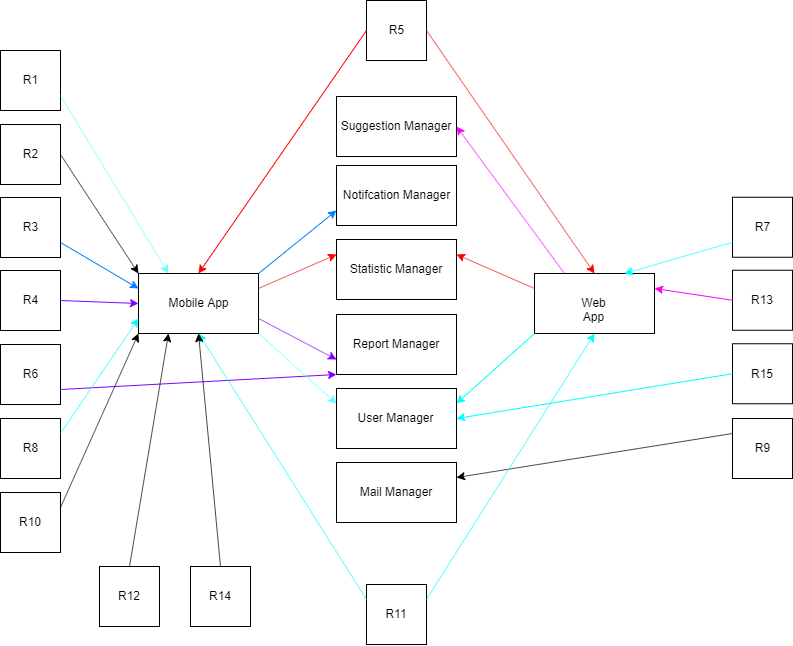
\includegraphics{Images/ReqMapping.png}
\end{figure}
%.-------------------------------------------------------------------------------------------------------------------------------------------------------------
